\documentclass[a4paper,hidelinks,12pt]{article}
\usepackage{amsmath,graphicx}
\usepackage[utf8]{inputenc}
\usepackage[russian]{babel}
\usepackage{indentfirst}
\usepackage{colortbl}
\usepackage{setspace}
\usepackage[noend]{algorithmic}
\usepackage[nottoc,notlot,notlof]{tocbibind}
\usepackage{amssymb}
\usepackage{amsmath}
\usepackage{graphicx}
\usepackage[left=3cm,right=1.5cm,top=2cm,bottom=2cm,bindingoffset=0cm]{geometry}
\setcounter{secnumdepth}{4}
\linespread{1.5}
\usepackage{xcolor}
\usepackage{pdfcomment}
\usepackage{titlesec}
\newcommand{\sectionbreak}{\clearpage}

\begin {document}
\begin {titlepage}
\thispagestyle{empty}

\begin{center}
\vspace{-1cm}

%
% No necessity to specify laboratory.
%

\includegraphics[width=0.5\textwidth]{msu}\\
Московский Государственный Университет им. М.В. Ломоносова\\
Факультет Вычислительной Математики и Кибернетики\\
Кафедра Автоматизации Систем Вычислительных Комплексов\\

\vspace{3cm}

{\Large Шпилевой Владислав Дмитриевич}

\vspace{1cm}

{\LARGE\bfseries Разработка и реализация алгоритма отложенного
обновления вторичных индексов на LSM-деревьях\\}

\vspace{1cm}

{\Large Магистерская диссертация}
\end{center}

\vfill

\begin{flushright}
\textbf {Научный руководитель:}\\
к.ф.-м.н. ассистент \\
Д.Ю.Волканов\\
\textbf {Научный консультант:}\\
К.А.Осипов\\
\vspace{10mm}
\end{flushright}

\vfill

\begin{center}
Москва, 2018
\end{center}

\end{titlepage}

\setcounter{page}{2}
\onehalfspacing

\begin{abstract}

В настоящее время растет популярность баз данных, хранящих данные на диске не в
виде традиционных B-деревьев и их производных, а в виде LSM деревьев. Главное
преимущество LSM деревьев в том, что их обновление всегда приводит только к
последовательной записи на диск, в отличие от B-деревьев. Это возможно благодаря
тому, что LSM дерево способно хранить множество версий одной и той же записи -
за счет этого при обновлении дерева не нужно точечно читать и удалять старые
данные - это происходит позже во время слияния уровней LSM дерева. Это работает,
когда в таблице только один индекс - первичный. При наличии вторичных индексов
LSM деревья лишаются преимуществ версионности, так как при обновлении дерева
нужно явно читать и удалять старые данные из всех вторичных индексов. В
настоящей работе представлен обзор существующих способов решения этой проблемы,
а также разработанная модификация LSM дерева, которая позволяет не делать явных
чтений и удалений старых данных из вторичных индексов. Проведенное
экспериментальное исследование нового LSM дерева показало прирост скорости на
порядок при наличии нескольких вторичных индексов.

\end{abstract}

\newpage
\tableofcontents

\newpage
\section{Введение}

\subsection{Цель работы}
Целью работы является увеличение скорости обновления базы данных, которая
хранит индексы таблиц в LSM деревьях при помощи модификации процедур обновления
и слияния уровней LSM дерева.

\subsection{Актуальность}
LSM (Log-Structured Merge) деревья были разработаны в 1990-х ~\cite{lsm-intro}
годах для задач с интенсивной записью, и использовались в файловых системах и
для резервного копирования. Но их применение в СУБД (Система Управления Базой
Данных) было ограничено из-за \textit {скрытых чтений}. Скрытыми называют
чтения, которые выполняются СУБД при обновлении данных, чтобы либо найти старые
данные и удалить их, либо чтобы проверить ограничения уникальности при вставке
новых данных. Значительная часть чтений в СУБД - скрытая, так как почти любое
обновление данных требует проверки различных ограничений и удаления старых
данных, и это почти ничего не стоит в B-деревьях, где для обновления данных в
любом случае нужно читать~\cite{btree-intro}. Но на LSM деревьях скрытые чтения
значительно снижают производительность, поскольку лишают их преимуществ
версионности данных, когда можно сохранять новые данные не читая и не удаляя
старые явно.

С появлением SSD (Solid-State Drive) дисков абсолютная скорость любых чтений и
записи возросла на порядки по сравнению со старыми механическими дисками, но
существенно увеличился разрыв между скоростями последовательной записи и
последовательного чтения~\cite{ssd-tradeof}. Благодаря тому, что LSM дерево
всегда выполняет запись на диск последовательно, а чтения из него на SSD по
скорости мало отличаются от B-дерева, LSM дерево стало одной из стандартных
структур данных для СУБД. Например, на момент написания работы LSM деревья уже
используются в LevelDB~\cite{leveldb}, RocksDB~\cite{rocksdb},
Cassandra~\cite{open-chan-ssd}, Tarantool~\cite{tarantool},
BigTable~\cite{open-chan-ssd}, HBase~\cite{open-chan-ssd}, Riak~\cite{riak},
MySQL~\cite{myrocks}.

Однако SSD хоть и делает LSM дерево более конкурентноспособным, но не решает
проблему существования скрытых чтений на любое обновление при наличии вторичных
индексов, что не позволяет использовать все возможности LSM деревьев, когда
в таблице в БД (База Данных) больше одного индекса.

Когда в таблице только один индекс на LSM дереве, то любые изменения, не
требующие знания старых данных (такие как \textit{REPLACE, DELETE}), возможны
без скрытых чтений. Например, в случае \textit{REPLACE} запись просто попадает
в дерево с новой версией. Тоже самое при \textit{DELETE} - ключ (набор
индексируемых колонок и их значений), по которому производится удаление,
попадает в дерево с новой версией и пометкой, что это именно удаление, а не
вставка. Скрытых чтений не выполняется. Но при появлении вторичного индекса даже
\textit{REPLACE} и \textit{DELETE} вынуждены читать старые данные из первичного
индекса, чтобы узнать, какой у старой записи был вторичный ключ, и вставить его
\textit{DELETE} в LSM дерево вторичного индекса.

Это обычная процедура для индексов на B-деревьях, где нет версионности данных, и
на классических LSM деревьях ее тоже нельзя избежать. Это происходит из-за того,
что удаление старых версий данных в LSM дереве работает так, что записи
считаются разными версиями одних и тех же данных, только если они равны по
ключу, по которому сортируется дерево. И если некоторый запрос меняет этот ключ
в уже существующей записи, не читая и не удаляя ее явно, то новая запись
становится никак не связанной со старой, и старая не удалится никогда - LSM
дерево видит их как разные ключи.

Таким образом, задача борьбы со скрытыми чтениями в таблицах с индексами на LSM
деревьях становится актуальной.

\subsection{Постановка задачи}
Разработать и реализовать алгоритм отложенного обновления вторичных индексов на
LSM-деревьях на основе базы данных Tarantool. Для достижения заданной цели
необходимо решить следующие подзадачи:
\begin{enumerate}
\item исследовать существующие способы уменьшения влияния скрытых чтений и
      ускорения записи;
\item разработать алгоритм отложенного обновления вторичных индексов на
      LSM-деревьях;
\item реализовать алгоритм на основе архитектуры базы данных Tarantool;
\item провести экспериментальную апробацию реализации.
\end{enumerate}

\subsection{Структура работы}
Во второй главе приведен обзор существующих способов уменьшения влияния скрытых
чтений на запись в БД, рассказано о том, какие у них недостатки и преимущества,
и почему их не достаточно для решения задачи.

Для более тонкого понимания актуальности проблемы скрытых чтений именно на LSM
деревьях в третьей главе раскрываются основные детали устройства LSM дерева,
кратко изложены алгоритмы его обновления (вставки, удаления, слияния уровней),
устройство индекса, хранящего данные в LSM дереве. В той же главе на примере
таблицы с множеством индексов на LSM деревьях разобрана проблема ее обновления.

В главе 4 описан предложенный алгоритм отложенного обновления индексов на LSM
деревьях. В этой главе детально разобран каждый шаг алгоритма, и приведены
математические доказательства ускорения записи. Здесь же разобрана реализация
новых LSM деревьев на архитектуре БД Tarantool.

В пятой главе представлены результаты экспериментального измерения
производительности новых таблиц на LSM деревьях в сравнении со старыми.

Последняя глава, шестая, содержит описание результатов работы, и рассуждения о
том, в какую сторону можно развивать новый алгоритм, и какие еще есть способы
ускорить запись в БД.

\section{Обзор существующих способов ускорения записи}
Цели обзора:
\begin{itemize}
\item показать, что проблема скрытых чтений появилась давно, действительно
актуальна до сих пор, и не только на LSM деревьях;
\item вычленить из существующих алгоритмов идеи, которые были бы применимы для
поставленной задачи;
\item учесть ошибки обозреваемых решений.
\end{itemize}

\subsection{Способ 1}
1

\subsection{Способ 2}
1

\subsection{Способ 3}
1


\section{LSM дерево}
LSM дерево~\cite{lsm-intro} - это структура данных, оптимизированная для задач с
интенсивной записью. Оно состоит из множества уровней: нулевой уровень хранится
в оперативной памяти, а остальные - на диске. В нулевой уровень записываются все
новые данные, обновления и удаления старых данных. Удаление в LSM дереве тоже
реализовано через вставку особой записи в нулевой уровень.

Когда нулевой уровень становится слишком велик, то он записывается на диск, и
удаляется из памяти. При этом запись нулевого уровня на диск выполняется
последовательно независимо от того, какие ключи, какие операции и в каком
порядке он содержит. Записанный уровень становится первым, и в памяти создается
новый пустой нулевой уровень для последующих обновлений.

При достижении числом уровней определенного порога LSM дерево выполняет
процедуру слияния уровней, во время которой некоторые соседние уровни
объединяются в один. LSM дерево может содержать разные версии одних и тех же
данных на разных уровнях, например, если запись с некоторым ключом сначала
вставили в нулевой уровень, затем он был записан на диск, и в новый нулевой
уровень было вставлено обновление или удаление по тому же ключу. Во время
слияния уровней старые версии записей обнаруживаются и удаляются - они просто не
попадают в новый уровень. То есть слияние в том числе выполняет функцию сборки
мусора. После окончания объединения старые уровни удаляются и заменяются одним
новым.

\begin{figure}
\centering
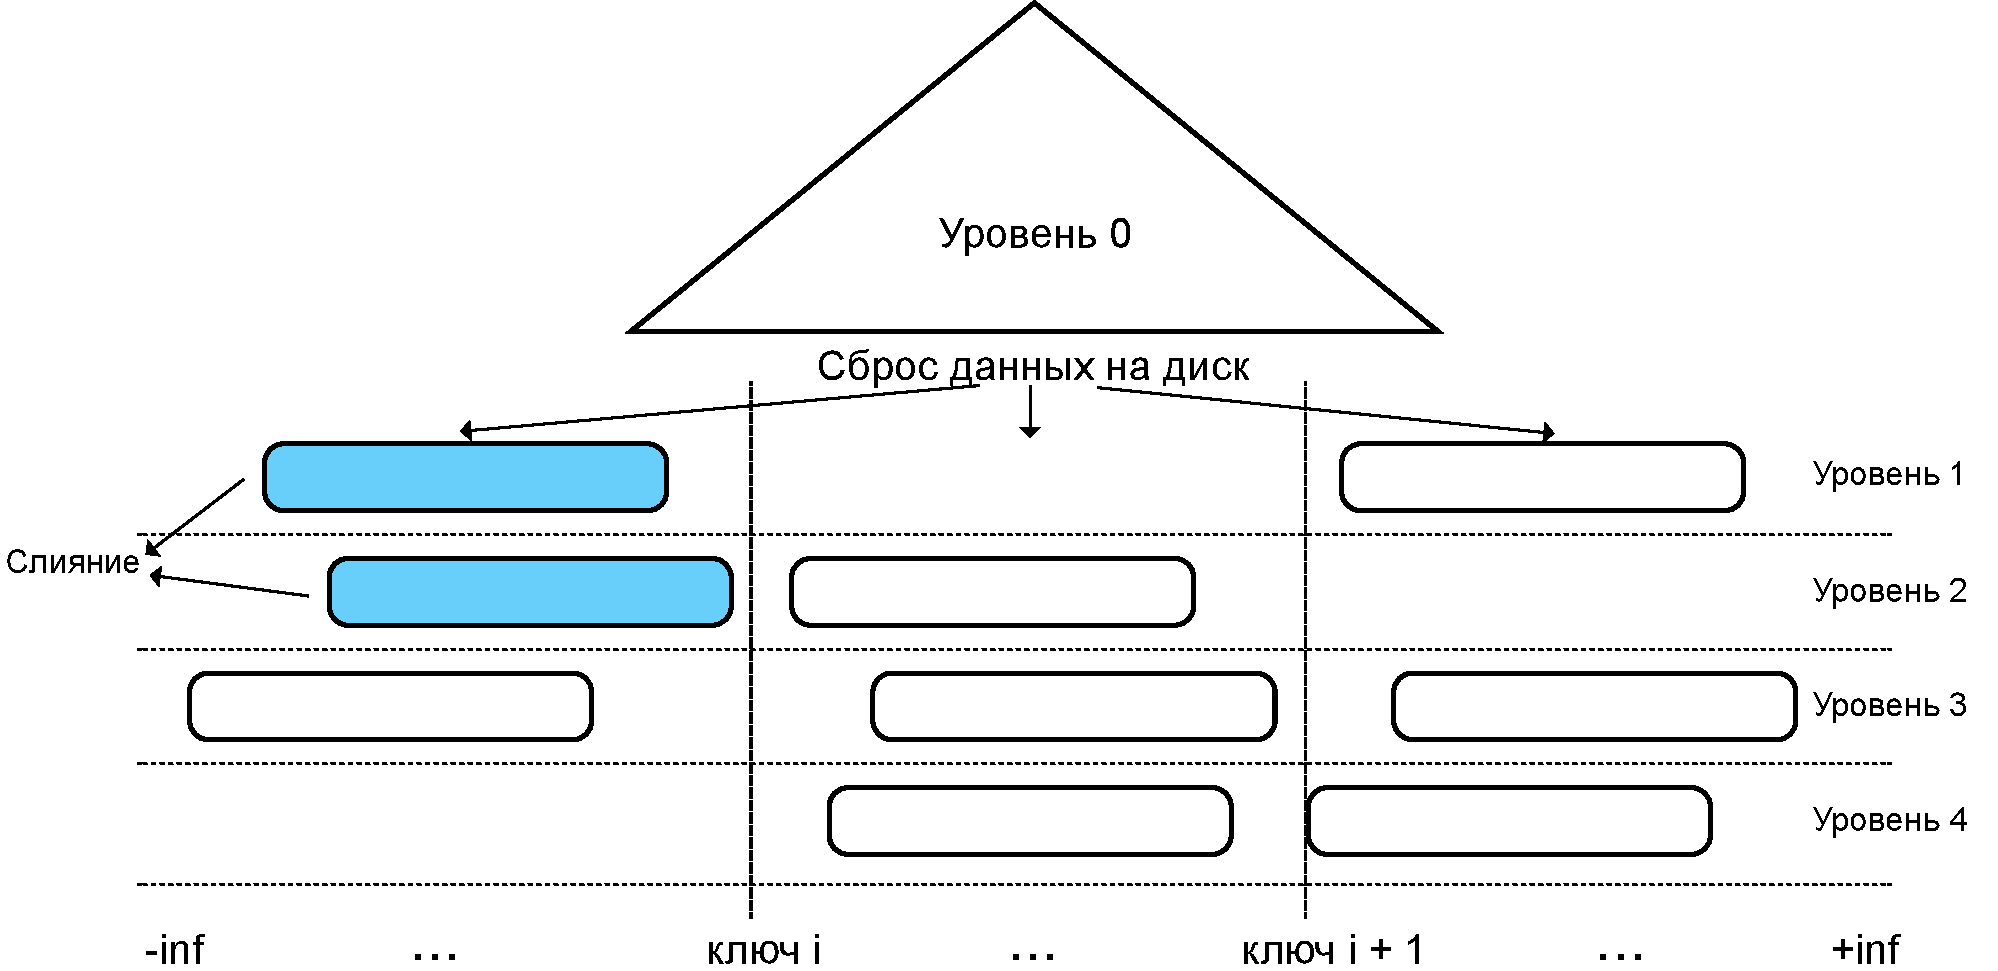
\includegraphics[width=0.7\textwidth]{compaction_schema}
\caption{Схематичное устройство LSM дерева с диапазонами}
\label{fig:compaction_schema}
\end{figure}

Способ организации нулевого уровня и уровней на диске не специфицируется явно,
и зависит от реализации. Например, нулевой уровень может быть организован как
B+ или красно-черное дерево. На диске уровни могут хранится в виде B деревьев,
или как просто массивы записей, отсортированные по ключу.

В данной работе рассматривается такая архитектура, при которой данные на диске
хранятся в виде отсортированных массивов, а в памяти в виде B+ дерева. Кроме
того, в рассматриваемом LSM дереве значения всех ключей, которые оно хранит,
разбиваются на диапазоны, каждый из которых содержит подуровни с данными его
ключей. Внутри диапазона подуровни могут объединяться независимо от других
диапазонов - это позволяет сделать процесс слияния уровней LSM дерева более
гранулярным. На рисунке~\ref{fig:compaction_schema} изображена схема дерева,
устроенного таким образом.

Описанный вариант LSM дерева не ограничивает общности алгоритма отложенного
обновления, вводимого в следующих главах, но позволяет рассматривать алгоритмы
работы с LSM деревом более конкретно в настоящей работе, и может быть применим к
другим вариациям LSM дерева.

\subsection{Слияние уровней}

Слияние уровней служит для уменьшения высоты дерева, и для удаления старых
версий записей. Оно выполняется на некотором подмножестве верхних уровней (при
этом возможна ситуация, когда объединяются все уровни дерева). Результатом
слияния является новый уровень LSM дерева, который по размеру не превышает
суммарного размера объединенных уровней, и заменяет их в дереве. Старые уровни
удаляются.

То, как именно выполняется слияние, зависит от реализации LSM дерева. Например,
на рассматриваемой здесь архитектуре, слияние выполняется не на целых уровнях, а
на подуровнях внутри каждого диапазона (на рисунке ~\ref{fig:compaction_schema}
изображен пример).

Некоторое множество верхних подуровней, представленных массивами записей,
отсортированных по ключу дерева, при помощи сортировки слияниями объединяется
в новый отсортированный массив. Сортировка слияниями гарантирует, что если
в разных источниках есть разные версии одной записи (то есть они равны по
ключу), то на некотором шаге сортировки можно будет увидеть их все разом, и в
этот момент понять, какая запись самая новая и попадет в новый массив, а какие
будут пропущены. Возможна ситуация, что ни одна из версий не попадет в новый
массив, если самая новая версия - это запись об удалении ключа.

Частота выполнения слияний уровней определяется несколькими параметрами дерева:
\begin{itemize}
\item коэффициент размера уровней - это такое число, что в каждой паре соседних
уровней $i$ и $i + 1$ размер уровня $i + 1$ должен быть как минимум в это число
раз больше, чем размер уровня $i$;
\item максимальная глубина дерева - это ограничение на максимальное число
уровней.
\end{itemize}

Если нарушено хотя бы одно из этих условий, то процедура слияния выполняется на
таком числе уровней, чтобы удовлетворить оба условия.

Слияние уровней на практике является дорогой процедурой, поскольку выполняются
чтение и запись диска (все уровни, кроме нулевого, хранятся на диске). Но так
как в LSM дереве данные не меняются на месте (вместо этого создаются новые
версии), то гарантируется, что уже записанные на диск уровни не изменятся, и это
позволяет выполнять процедуру слияния уровней в фоне и одновременно с их чтением
различными пользовательскими запросами. Архитектура с разбиением значений ключей
дерева на диапазоны открывает возможность выполнения одновременных слияний в
разных диапазонах.

\subsection{Индексы на LSM деревьях}

LSM деревья, помимо прочих применений, используются для хранения индексов в
базах данных~\cite{leveldb, rocksdb, tarantool}. Дерево такого индекса
сортируется по его ключевым полям. При этом одна таблица может иметь несколько
индексов - один первичный и некоторое число вторичных.

Первичный индекс всегда уникален, а записи такого индекса хранят каждую запись
целиком в том виде, в котором она попала в таблицу. Вторичный индекс хранит свой
ключ объединенный с первичным ключом, и не хранит всю остальную часть записи.
Это позволяет экономить память, храня не влияющую на сортировку часть записи
только один раз - в первичном индексе. Первичный ключ в записях вторичного
индекса используется, чтобы по любой записи во вторичном индексе можно было
найти ее полную версию в первичном, когда запрос выполняет поиск по вторичному
индексу.

Описанная архитектура индексов не является уникальной для LSM деревьев. Индексы
на B и B+ деревьях могут хранится таким же
образом~\cite{secondary-search, sqlite}: полная запись в первичном индексе, и
только ключевые части во вторичных.

Поскольку вторичные индексы связаны с первичным, СУБД должна поддерживать
консистентность индексов - если записи нет в первичном, то ее не должно быть ни
в одном из вторичных. И наоборот - если запись есть в первичном, то она должна
существовать в каждом вторичном индексе. Именно по этой причине существует
необходимость в скрытых чтениях - если обновление таблицы изменяет вторичный
ключ некоторой записи, или вовсе ее удаляет, то это нужно отразить во всех
вторичных индексах, для чего выполняется чтение полной записи из первичного
индекса и удаление старых ключей из других индексов. Иначе нарушается
консистентность.

\subsection{Проблема обновления индексов}

\begin{figure}
\centering
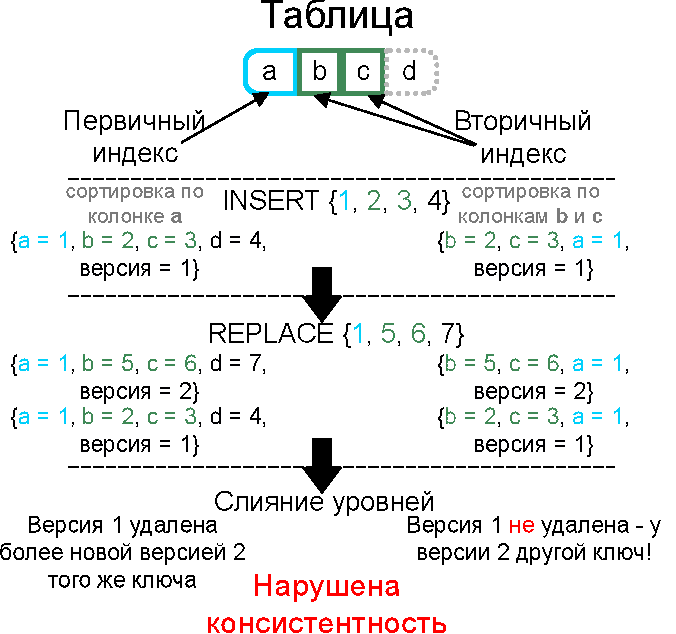
\includegraphics[width=0.45\textwidth]{inconsistent_example}
\caption{Пример нарушения консистентности в LSM индексах}
\label{fig:inconsistent_example}
\end{figure}

Способность LSM дерева хранить множество версий одного ключа позволяет избегать
скрытых чтений на такие операции как \textit{REPLACE} и \textit{DELETE},
которые не могут нарушить консистентность на таблице с единственным индексом и
без внешних ключей (FOREIGN KEY). Эти операции называются
\textit {слепой записью}~\cite{slimdb}. Слепая запись всегда значительно
быстрее, чем операции вроде \textit{INSERT} или \textit{UPDATE}, которые в
худшем случае обращаются к диску, чтобы проверить ограничения уникальности, или
чтобы прочитать полную запись для выполнения обновления.

Проблема обновления индексов таблицы на LSM деревьях состоит в том, что при
наличии вторичных индексов слепая запись становится невозможна ни для каких
операций. На рисунке~\ref{fig:inconsistent_example} изображен пример нарушения
консистентности, к которому может привести слепой \textit{REPLACE} во вторичный
индекс. В примере у таблицы 4 колонки: первая - ключ первичного индекса,
вторая и третья - ключ вторичного индекса, и четвертая не используется в
индексах. Перед выполнением \textit{REPLACE{1, 5, 6, 7}} должен прочесть старую
запись из первичного индекса по ключу \textit{{1}}, извлечь вторичный ключ
\textit{{2, 3}}, удалить его из вторичного индекса, и только затем вставлять
везде новую запись. Если старую запись из вторичного индекса не удалить явно,
то во время слияния уровней она становится мусором, у которого больше нет ссылки
на полную запись в первичном индексе. Но и удалить этот мусор нельзя, так как
более новая запись с тем же первичным ключом имеет другой вторичный ключ.
Сравнить их по первичному ключу в общем случае невозможно, так как индекс
отсортирован в первую очередь по вторичному ключу, и во время слияний уровней
эти записи могут никогда не встретиться.

Поскольку доступ к диску всегда намного медленнее, чем доступ к памяти, то
наличие вторичных индексов делает версионность LSM дерева бесполезной - неявное
удаление старых версий ключа более новыми версиями не работает. В следующей
главе представлен алгоритм обновления LSM индексов, который возвращает записи
слепоту.

\section{Отложенное обновление вторичных индексов на LSM деревьях}
1

\subsection{Вставка и удаление}
1

\subsection{Слияние уровней}
1

\subsubsection{Первичный индекс}
1

\subsubsection{Вторичный индекс}
1

\subsection{Чтения}
1

\subsection{Реализация}
1


\section{Экспериментальное исследование}
1


\section{Заключение}
1

\begin{thebibliography}{9}

\bibitem{lsm-intro} O’Neil P. et al. The log-structured merge-tree (LSM-tree) //Acta Informatica. – 1996. – Т. 33. – No. 4. – С. 351-385.
\bibitem{btree-intro} Comer D. Ubiquitous B-tree //ACM Computing Surveys (CSUR). – 1979. – Т. 11. – №. 2. – С. 121-137.
\bibitem{ssd-tradeof} Agrawal N. et al. Design Tradeoffs for SSD Performance //USENIX Annual Technical Conference. – 2008. – Т. 8. – С. 57-70.
\bibitem{leveldb} Wang P. et al. An efficient design and implementation of LSM-tree based key- value store on open-channel SSD //Proceedings of the Ninth European Conference on Computer Systems. – ACM, 2014. – С. 16.
\bibitem{rocksdb} Yang F. et al. Optimizing NoSQL DB on flash: A case study of RocksDB //Ubiquitous Intelligence and Computing and 2015 IEEE 12th Intl Conf on Autonomic and Trusted Computing and 2015 IEEE 15th Intl Conf on Scalable Computing and Communications and Its Associated Workshops (UIC-ATC- ScalCom), 2015 IEEE 12th Intl Conf on. – IEEE, 2015. – С. 1062-1069.
\bibitem{open-chan-ssd} Wang P. et al. An efficient design and implementation of LSM-tree based key- value store on open-channel SSD //Proceedings of the Ninth European Conference on Computer Systems. – ACM, 2014. – С. 16.й
\bibitem{tarantool} Сайт базы данных Tarantool [Электронный ресурс] : сайт содержит документацию всех выпущенных версий Tarantool. — Режим доступа: https://tarantool.io. - Загл. с экрана.
\bibitem{riak} Lersch L. et al. An analysis of LSM caching in NVRAM //Proceedings of the 13th International Workshop on Data Management on New Hardware. – ACM, 2017. – С. 9.
\bibitem{myrocks} Dong S. et al. Optimizing Space Amplification in RocksDB //CIDR. – 2017.
\bibitem{secondary-search} Liu L. C. H., Yoneda K. Secondary index search : пат. 6266660 США. – 2001.
\bibitem{sqlite} Owens M., Allen G. SQLite. – Apress LP, 2010.
\bibitem{slimdb} Ren K. et al. SlimDB: a space-efficient key-value storage engine for semi-sorted data //Proceedings of the VLDB Endowment. – 2017. – Т. 10. – №. 13. – С. 2037-2048.

\end{thebibliography}
\end{document}
